\documentclass[10pt]{article}
\usepackage[T1]{fontenc}

% Document Details
\newcommand{\CLASS}{AMATH 584}
\newcommand{\assigmentnum}{Assignment 6}

\usepackage[margin = 1.15in, top = 1.25in, bottom = 1.in]{geometry}

\usepackage{titling}
\setlength{\droptitle}{-6em}   % This is your set screw
\date{}
\renewcommand{\maketitle}{
	\clearpage
	\begingroup  
	\centering
	\LARGE \sffamily\textbf{\CLASS} \Large \assigmentnum\\[.8em]
	\large Tyler Chen\\[1em]
	\endgroup
	\thispagestyle{empty}
}
 % Title Styling
\usepackage{tocloft}
\renewcommand{\cfttoctitlefont}{\Large\sffamily\bfseries}
\renewcommand{\cftsecfont}{\normalfont\sffamily\bfseries}
\renewcommand{\cftsubsecfont}{\normalfont\sffamily}
\renewcommand{\cftsubsubsecfont}{\normalfont\sffamily}

\makeatletter
\let\oldl@section\l@section
\def\l@section#1#2{\oldl@section{#1}{\sffamily\bfseries#2}}

\let\oldl@subsection\l@subsection
\def\l@subsection#1#2{\oldl@subsection{#1}{\sffamily#2}}

\let\oldl@subsubsection\l@subsubsection
\def\l@subsubsection#1#2{\oldl@subsubsection{#1}{\sffamily#2}}
 % General Styling


\usepackage{enumitem}

% Figures
\usepackage{subcaption}

% TikZ and Graphics
\usepackage{tikz, pgfplots}
\pgfplotsset{compat=1.12}
\usetikzlibrary{patterns,arrows}
\usepgfplotslibrary{fillbetween}

\usepackage{pdfpages}
\usepackage{adjustbox}

\usepackage{lscape}
\usepackage{titling}
\usepackage[]{hyperref}


% Header Styling
\usepackage{fancyhdr}
\pagestyle{fancy}
\lhead{\sffamily \CLASS}
\rhead{\sffamily Chen \textbf{\thepage}}
\cfoot{}

% Paragraph Styling
\setlength{\columnsep}{1cm}
\setlength{\parindent}{0pt}
\setlength{\parskip}{5pt}
\renewcommand{\baselinestretch}{1}

% TOC Styling
\usepackage{tocloft}
\iffalse
\renewcommand{\cftsecleader}{\cftdotfill{\cftdotsep}}

\renewcommand\cftchapafterpnum{\vskip6pt}
\renewcommand\cftsecafterpnum{\vskip10pt}
\renewcommand\cftsubsecafterpnum{\vskip6pt}

% Adjust sectional unit title fonts in ToC
\renewcommand{\cftchapfont}{\sffamily}
\renewcommand{\cftsecfont}{\bfseries\sffamily}
\renewcommand{\cftsecnumwidth}{2em}
\renewcommand{\cftsubsecfont}{\sffamily}
\renewcommand{\cfttoctitlefont}{\hfill\bfseries\sffamily\MakeUppercase}
\renewcommand{\cftaftertoctitle}{\hfill}

\renewcommand{\cftchappagefont}{\sffamily}
\renewcommand{\cftsecpagefont}{\bfseries\sffamily}
\renewcommand{\cftsubsecpagefont}{\sffamily}
\fi
 % General Styling
% Code Display Setup
\usepackage{listings,lstautogobble}
\usepackage{lipsum}
\usepackage{courier}
\usepackage{catchfilebetweentags}

\lstset{
	basicstyle=\small\ttfamily,
	breaklines=true, 
	frame = single,
	rangeprefix=,
	rangesuffix=,
	includerangemarker=false,
	autogobble = true
}


\usepackage{algorithmicx}
\usepackage{algpseudocode}

\newcommand{\To}{\textbf{to}~}
\newcommand{\DownTo}{\textbf{downto}~}
\renewcommand{\algorithmicdo}{\hspace{-.2em}\textbf{:}}
 % Code Display Setup
% AMS MATH Styling
\usepackage{amsmath, amssymb}
\newcommand{\qed}{\hfill\(\square\)}

%\newtheorem*{lemma}{Lemma} 
%\newtheorem*{theorem}{Theorem}
%\newtheorem*{definition}{Definition}
%\newtheorem*{prop}{Proposition}
%\renewenvironment{proof}{{\bfseries Proof.}}{}


% mathcal
\newcommand{\cA}{\ensuremath{\mathcal{A}}}
\newcommand{\cB}{\ensuremath{\mathcal{B}}}
\newcommand{\cC}{\ensuremath{\mathcal{C}}}
\newcommand{\cD}{\ensuremath{\mathcal{D}}}
\newcommand{\cE}{\ensuremath{\mathcal{E}}}
\newcommand{\cF}{\ensuremath{\mathcal{F}}}
\newcommand{\cG}{\ensuremath{\mathcal{G}}}
\newcommand{\cH}{\ensuremath{\mathcal{H}}}
\newcommand{\cI}{\ensuremath{\mathcal{I}}}
\newcommand{\cJ}{\ensuremath{\mathcal{J}}}
\newcommand{\cK}{\ensuremath{\mathcal{K}}}
\newcommand{\cL}{\ensuremath{\mathcal{L}}}
\newcommand{\cM}{\ensuremath{\mathcal{M}}}
\newcommand{\cN}{\ensuremath{\mathcal{N}}}
\newcommand{\cO}{\ensuremath{\mathcal{O}}}
\newcommand{\cP}{\ensuremath{\mathcal{P}}}
\newcommand{\cQ}{\ensuremath{\mathcal{Q}}}
\newcommand{\cR}{\ensuremath{\mathcal{R}}}
\newcommand{\cS}{\ensuremath{\mathcal{S}}}
\newcommand{\cT}{\ensuremath{\mathcal{T}}}
\newcommand{\cU}{\ensuremath{\mathcal{U}}}
\newcommand{\cV}{\ensuremath{\mathcal{V}}}
\newcommand{\cW}{\ensuremath{\mathcal{W}}}
\newcommand{\cX}{\ensuremath{\mathcal{X}}}
\newcommand{\cY}{\ensuremath{\mathcal{Y}}}
\newcommand{\cZ}{\ensuremath{\mathcal{Z}}}

% mathbb
\usepackage{bbm}
\newcommand{\bOne}{\ensuremath{\mathbbm{1}}}

\newcommand{\bA}{\ensuremath{\mathbb{A}}}
\newcommand{\bB}{\ensuremath{\mathbb{B}}}
\newcommand{\bC}{\ensuremath{\mathbb{C}}}
\newcommand{\bD}{\ensuremath{\mathbb{D}}}
\newcommand{\bE}{\ensuremath{\mathbb{E}}}
\newcommand{\bF}{\ensuremath{\mathbb{F}}}
\newcommand{\bG}{\ensuremath{\mathbb{G}}}
\newcommand{\bH}{\ensuremath{\mathbb{H}}}
\newcommand{\bI}{\ensuremath{\mathbb{I}}}
\newcommand{\bJ}{\ensuremath{\mathbb{J}}}
\newcommand{\bK}{\ensuremath{\mathbb{K}}}
\newcommand{\bL}{\ensuremath{\mathbb{L}}}
\newcommand{\bM}{\ensuremath{\mathbb{M}}}
\newcommand{\bN}{\ensuremath{\mathbb{N}}}
\newcommand{\bO}{\ensuremath{\mathbb{O}}}
\newcommand{\bP}{\ensuremath{\mathbb{P}}}
\newcommand{\bQ}{\ensuremath{\mathbb{Q}}}
\newcommand{\bR}{\ensuremath{\mathbb{R}}}
\newcommand{\bS}{\ensuremath{\mathbb{S}}}
\newcommand{\bT}{\ensuremath{\mathbb{T}}}
\newcommand{\bU}{\ensuremath{\mathbb{U}}}
\newcommand{\bV}{\ensuremath{\mathbb{V}}}
\newcommand{\bW}{\ensuremath{\mathbb{W}}}
\newcommand{\bX}{\ensuremath{\mathbb{X}}}
\newcommand{\bY}{\ensuremath{\mathbb{Y}}}
\newcommand{\bZ}{\ensuremath{\mathbb{Z}}}

% alternative mathbb
\newcommand{\NN}{\ensuremath{\mathbb{N}}}
\newcommand{\RR}{\ensuremath{\mathbb{R}}}
\newcommand{\CC}{\ensuremath{\mathbb{C}}}
\newcommand{\ZZ}{\ensuremath{\mathbb{Z}}}
\newcommand{\EE}{\ensuremath{\mathbb{E}}}
\newcommand{\PP}{\ensuremath{\mathbb{P}}}
\newcommand{\VV}{\ensuremath{\mathbb{V}}}
\newcommand{\cov}{\ensuremath{\text{Co}\VV}}
% Math Commands

\newcommand{\st}{~\big|~}
\newcommand{\stt}{\text{ st. }}
\newcommand{\ift}{\text{ if }}
\newcommand{\thent}{\text{ then }}
\newcommand{\owt}{\text{ otherwise }}

\newcommand{\norm}[1]{\left\lVert#1\right\rVert}
\newcommand{\snorm}[1]{\lVert#1\rVert}
\newcommand{\ip}[1]{\ensuremath{\left\langle #1 \right\rangle}}
\newcommand{\pp}[3][]{\frac{\partial^{#1}#2}{\partial #3^{#1}}}
\newcommand{\dd}[3][]{\frac{\d^{#1}#2}{\d #3^{#1}}}
\renewcommand{\d}{\ensuremath{\mathrm{d}}}

\newcommand{\indep}{\rotatebox[origin=c]{90}{$\models$}}




 % Math shortcuts
% Problem
\usepackage{floatrow}

\newenvironment{problem}[1][]
{\pagebreak
\noindent\rule{\textwidth}{1pt}\vspace{0.25em}
{\sffamily \textbf{#1}}
\par
}
{\par\vspace{-0.5em}\noindent\rule{\textwidth}{1pt}}

\newenvironment{solution}[1][]
{{\sffamily \textbf{#1}}
\par
}
{}

 % Problem Environment

\newcommand{\note}[1]{\textcolor{red}{\textbf{Note:} #1}}

\hypersetup{
   colorlinks=true,       % false: boxed links; true: colored links
   linkcolor=violet,          % color of internal links (change box color with linkbordercolor)
   citecolor=green,        % color of links to bibliography
   filecolor=magenta,      % color of file links
   urlcolor=cyan           % color of external links
}


\begin{document}
\maketitle

\begin{problem}[Exercise 1]
Let \(A\) be an \(m\) by \(m\) nonsingular matrix and let \(b\) be a given nonzero \(m\)-vector.  Suppose \(x\) satisfies \(Ax = b\) and \(\hat{x}\) satisfies \(A \hat{x} = \hat{b}\), where \(\hat{b}\) is slightly different from \(b\).  Show that
\[ \frac{\| \hat{x} - x \|_2}{\| x \|_2} \leq \kappa (A) \frac{\| \hat{b} - b \|_2}
{\| b \|_2} ,\]
where \(\kappa (A) = \| A \|_2 \| A^{-1} \|_2\) is the 2-norm condition number of \(A\).  Show that there are nonzero vectors \(b\) and \(\hat{b} - b\) for which equality holds.  [Note:  You might want to review material in Lecture 12 of the text.]
\end{problem}

\begin{solution}[Solution]
We have \( Ax=b \) and \( A\hat{x} = \hat{b} \) so that \( A(\hat{x}-x) = A\hat{x} -Ax = \hat{b}-b \). Since \( A \) is nonsingular, we have \( \hat{x}-x = A^{-1}(\hat{b}-b) \).

Then, \( \norm{b}_2 = \norm{Ax}_2 \leq \norm{A}_2\norm{x}_2 \) and \( \norm{\hat{x}-x}_2 = \snorm{A^{-1}(\hat{b}-b)}_2 \leq \snorm{A^{-1}}_2\snorm{\hat{b}-b}_2 \). Rearranging the first equation we have \( 1/\norm{x}_2 \leq \norm{A}_2/\norm{b}_2 \).
Therefore,
\begin{align*}
    \dfrac{\norm{\hat{x}-x}_2}{\norm{x}_2} \leq \norm{A}_2\norm{A^{-1}}_2\dfrac{\snorm{\hat{b}-b}_2}{\norm{b}_2} = \kappa(A) \dfrac{\snorm{\hat{b}-b}_2}{\norm{b}_2} \tag*{\qed}
\end{align*}

Recall the first right singular vector \( v_1 \) of a matrix \( A \) satisfies \( \norm{A} = \norm{Av}/\norm{v} \) so that \( \norm{A}\norm{v} = \norm{Av} \).

Then take \( x \) as the first right singular vector of \( A \) and \( b=Ax \) so that \( \norm{b}_2 = \norm{A}_2\norm{x}_2 \). Likewise, take \( (\hat{b}-b) \) as the first right singular vector of \( A^{-1} \) so that \( \snorm{\hat{x}-x}_2 = \norm{A^{-1}}_2\snorm{\hat{b}-b}_2 \). Then,
\begin{align*}
    \dfrac{\norm{\hat{x}-x}_2}{\norm{x}_2} = \norm{A}_2\norm{A^{-1}}_2\dfrac{\snorm{\hat{b}-b}_2}{\norm{b}_2} = \kappa(A) \dfrac{\snorm{\hat{b}-b}_2}{\norm{b}_2} \tag*{\qed} 
\end{align*} 
\end{solution}


\begin{problem}[Exercise 2]
The idea of this exercise is to carry out an experiment analogous to the one described
in Lec. 16 of the text, but for the SVD instead of QR factorization.
\begin{enumerate}
    \item[(a)]
Write a program that constructs a \(50 \times 50\) matrix \verb+A = U*S*V'+,
where \verb+U+ and \verb+V+ are random orthogonal matrices and \verb+S+ is a diagonal
matrix whose diagonal entries are uniformly distributed numbers in \([0,1]\), sorted into
nonincreasing order.  You can use the following lines in MATLAB:

\begin{verbatim}
[U,X] = qr(randn(50));
[V,X] = qr(randn(50));
S = diag(sort(rand(50,1),'descend'));
A = U*S*V';
\end{verbatim}

Compute the SVD of \(A\):  \verb+[U2,S2,V2] = svd(A);+  Recall that the SVD of a real square
matrix is not quite uniquely determined.  Make sure that the signs of the columns of \verb+U2+
and \verb+V2+ match those of \verb+U+ and \verb+V+ as follows:

\begin{verbatim}
for j=1:50,
  if U2(:,j)'*U(:,j) < 0,   % The signs are different for the jth column.
    U2(:,j) = -U2(:,j); V2(:,j) = -V2(:,j);     % Change them to match.
  end;
end;
\end{verbatim}

Now compute \verb+norm(U2-U)+, \verb+norm(V2-V)+, \verb+norm(S2-S)/norm(S)+, and
\newline
\verb+norm(A - U2*S2*V2')/norm(A)+.  Run your program with five different random matrices
and comment on whether the various differences seem to be connected with the
condition number of \(A\), \verb+cond(A)+.

\item[(b)]
For each of the matrices in part(a), replace the diagonal entries in \verb+S+ by
their sixth powers (thus making the condition number of \verb+A+ much larger) and
repeat the experiment.  Do you see significant differences between these results and
those of the experiment for QR factorization in the text?
\end{enumerate}
\end{problem}

\begin{solution}[Solution]
We implement this in python as,
\begin{lstlisting}
def exercise_2():
    out=[]
    n=50
    [U,X]=np.linalg.qr(np.random.randn(n,n))
    [V,X]=np.linalg.qr(np.random.randn(n,n))
    ss=np.sort(np.random.rand(n))
    SS = [np.diag(np.flip(ss,0)), 
          np.diag(np.flip(ss**6,0))]
    
    for i in range(2):
        S= SS[i]
        A=U@S@V
        
        [U2,S2,V2]=np.linalg.svd(A,full_matrices=True)
        S2=np.diag(S2)
        
        for j in range(n):
            if np.dot(U2[:,j],U[:,j])<0:
                U2[:,j] = -U2[:,j]
                V2[j,:] = -V2[j,:]
        res=[np.linalg.norm(U2-U),
             np.linalg.norm(V2-V),
             np.linalg.norm(S2-S)/np.linalg.norm(S),
             np.linalg.norm(A-U2@S2@V2),
             np.linalg.cond(A)]
        out.append(res)
    return out 
\end{lstlisting}
\begin{enumerate}
    \item[(a)] 
        We test with 50 matrices as follows:
        \begin{lstlisting}
for i in range(4):
    plt.scatter(x[:,0,4], np.log10(x[:,0,i]))
    plt.scatter(x[:,1,4], np.log10(x[:,1,i]))
    plt.show()
        \end{lstlisting}
    It doesn't seem like there is a correlation between the condition number and the output.
    \item[(b)] 
        The plots show no clear relationship between the condition number and the norms, other than that \( U_2, V_2, S_2 \) are slightly less accurate as the condition number increases. Strangely, it seems that \( U_2S_2V_2 \) is marginally more accurate as the condition number increases.

        \begin{figure}[H]\centering
            \begin{subfigure}{.45\textwidth}\centering
                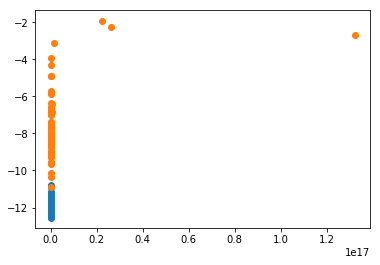
\includegraphics[width=.9\textwidth]{img/U2U.png}
                \caption{\(\norm{U_2-U}\) vs \( \kappa(A) \)}
            \end{subfigure}            
            \begin{subfigure}{.45\textwidth}\centering
                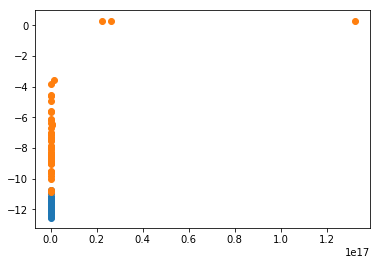
\includegraphics[width=.9\textwidth]{img/V2V.png}
                \caption{\(\norm{V_2-V}\) vs \( \kappa(A) \)}
            \end{subfigure}            
            \begin{subfigure}{.45\textwidth}\centering
                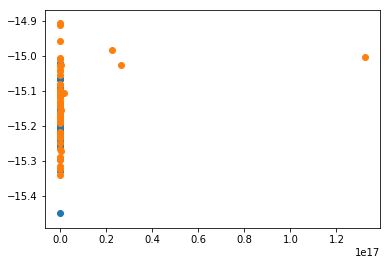
\includegraphics[width=.9\textwidth]{img/S2S.png}
                \caption{\(\norm{S_2-S}/\norm{S}\) vs \( \kappa(A) \)}
            \end{subfigure}            
            \begin{subfigure}{.45\textwidth}\centering
                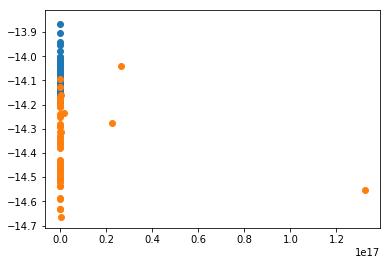
\includegraphics[width=.9\textwidth]{img/AUSV.png}
                \caption{\(\norm{A-USV^T}\) vs \( \kappa(A) \)}
            \end{subfigure}
            \caption{orange: higher condition number runs}
        \end{figure}

However, in the QR factorization from the text was unstable and resulted in bad results as the condition number increase. 

In particular, the Q and R factors were very off, although the product was not. 
Again we have the errors in \( U_2 \) and \( V_2\) about \( 10^{-8} \) although the product \( U_2S_2V_2 \) has error of about \( 10^{-14} \).

Note that there are some outputs of the norm function which give exactly 2.0. This seems to be a numerical error in the implementation of the 2-norm in numpy for matrices with norms very close to zero.

\end{enumerate}
\end{solution}


\begin{problem}[Exercise 3]
Write the following matrix in the form \(LU\), where \(L\) is a unit lower
triangular matrix and \(U\) is an upper triangular matrix:
\[
\left[ \begin{array}{rrr} 4 & -1 & -1 \\ -1 & 4 & -1 \\ -1 & -1 & 4 \end{array} \right] 
\]
Without completely redoing the calculation, write the same matrix in the form \(L L^T\), 
where \(L\) is lower triangular.  Explain how you can derive the \(L L^T\)-factorization
from the \(LU\) factorization, and vice-versa.
\end{problem}

\begin{solution}[Solution]
We apply row operations to zero the first entry in the second and third rows.
\begin{align*}
\left[ \begin{array}{rrr} 1 & 0 & 0 \\ 1/4 & 1 & 0 \\ 1/4 & 0 & 1 \end{array} \right] 
\left[ \begin{array}{rrr} 4 & -1 & -1 \\ -1 & 4 & -1 \\ -1 & -1 & 4 \end{array} \right]  = 
\left[ \begin{array}{rrr} 4 & -1 & -1 \\ 0 & 15/4 & -5/4 \\ 0 & -5/4 & 15/4 \end{array} \right] 
\end{align*}

We apply row operators to zero the second entry in the third row.
\begin{align*}
\left[ \begin{array}{rrr} 1 & 0 & 0 \\ 0 & 1 & 0 \\ 0 & 1/3 & 1 \end{array} \right] 
\left[ \begin{array}{rrr} 4 & -1 & -1 \\ 0 & 15/4 & -5/4 \\ 0 & -5/4 & 15/4 \end{array} \right] =
\left[ \begin{array}{rrr} 4 & -1 & -1 \\ 0 & 15/4 & -5/4 \\ 0 & 0 & 10/3 \end{array} \right]
\end{align*}

Thus,
\begin{align*}
    L =
    \left(
    \left[ \begin{array}{rrr} 1 & 0 & 0 \\ 0 & 1 & 0 \\ 0 & 1/3 & 1 \end{array} \right] 
    \left[ \begin{array}{rrr} 1 & 0 & 0 \\ 1/4 & 1 & 0 \\ 1/4 & 0 & 1 \end{array} \right]
        \right)^{-1} =
    \left[ \begin{array}{rrr} 1 & 0 & 0 \\ 1/4 & 1 & 0 \\ 1/4 & 1/3 & 1 \end{array} \right]^{-1} = 
        \left[\begin{array}{rrr} 1 & 0 & 0 \\ -1/4 & 1 & 0 \\ -1/4 & -1/3 & 1  \end{array}\right]
\end{align*}

And,
\begin{align*}
    U= 
\left[ \begin{array}{rrr} 4 & -1 & -1 \\ 0 & 15/4 & -5/4 \\ 0 & 0 & 10/3 \end{array} \right] 
\end{align*}

To go from a LU decomposition to a \( LL^T \) transition first take the diagonal entries of \( U \).
\begin{align*}
    D = \left[\begin{array}{rrr}4 && \\ & 15/4 &\\ & & 10/3\end{array}\right]
\end{align*}

We then rewrite \( U = DU' \) with unit lower triangular matrix \( U' = L^T \) and a diagonal matrix \( D^{-1} \).
\begin{align*}
    U' = D^{-1}U = \left[\begin{array}{rrr}1/4 & & \\ & 4/15 & \\ & & 3/10\end{array}\right]    
\left[ \begin{array}{rrr} 4 & -1 & -1 \\ 0 & 15/4 & -5/4 \\ 0 & 0 & 10/3 \end{array} \right] = 
    \left[\begin{array}{rrr}1 & -1/4 & -1/4 \\ 0 & 1 &  -1/3 \\ 0 & 0 & 1\end{array}\right] 
    =L^T
\end{align*}

    Then, \( A = LDL^T \). Now rewrite \( D \) as the square of a diagonal matrix denoted \( \sqrt{D} \). In particular,
\begin{align*}
    \sqrt{D} = \left[\begin{array}{rrr} \sqrt{4} && \\ & \sqrt{15/4} &\\ & & \sqrt{10/3}\end{array}\right]
\end{align*}

Then let,
\begin{align*}
    L' = L\sqrt{D} =
    \left[\begin{array}{rrr} 1 & 0 & 0 \\ -1/4 & 1 & 0 \\ -1/4 & -1/3 & 1  \end{array}\right]
    \left[\begin{array}{rrr} \sqrt{4} && \\ & \sqrt{15/4} &\\ & & \sqrt{10/3}\end{array}\right] = 
        \left[\begin{array}{rrr} 2 & 0 & 0 \\-1/2 & \sqrt{15/4} & 0 \\ -1/2 & -\sqrt{5/12} & \sqrt{10/3} \end{array}\right]
\end{align*}

Thus, 
\begin{align*}
    (L')(L')^T = (L\sqrt{D})(\sqrt{D}^TL^T) = L D L^T = L U = A 
\end{align*}

To return from a \( LL^T \) decomposition, first factor \( L \) into a lower unit triangular matrix by the method shown above, and then left multiply \( L^T \) by the appropriate factor. That is, let \( D \) be a diagonal matrix with the diagonal entires of \( L \). Then \( LD^{-1} \) is unit lower triangular, so \( (LD^{-1}) (DL^T) \) is a LU decomposition. 

\end{solution}


\begin{problem}[Exercise 20.1]
    Let \( A\in\CC^{m\times  m} \) be nonsingular. Show that \( A \) has an LU factorization if and only if for each \( k \) with \( 1\leq k\leq m \), the upper-left \( k\times k \) block \( A_{1:k,1:k} \) is nonsingular. Prove this LU factorization is unique.
    Hint: The row operations of Gaussian eliminiation leave the determindants \( \det(A_{1:k,1:k}) \) unchanged.
\end{problem}

\begin{solution}[Solution]
Since \( A \) is nonsingular, \( \det(A)\neq 0 \). 

Suppose each block \( A_{1:k,1:k} \) is nonsingular for \( 1\leq k\leq m \).

Since \( A_{1:1,1:1} \) is nonsingular, the first pivot position is nonzero, so we can zero the entries below the pivot. In the second step, \( A^{(1)}_{1:2,1:2} \) is nonsingular, so \( A_{2,2} \) is nonzero so we can again pivot. Repeating this argument means we can perform the Gaussian elimination algorithm without partial pivoting and it will not fail.  So \( A \) has a LU decomposition.


Now, suppose \( A \) has an LU decomposition. Then \( 0\neq \det(A) = \det(L)\det(U) \). The determinant of a triangular matrix is the product of the diagonal entries so \( U \) has no zeros on the diagonals. Thus, \( \det(L_{1:k,1:k})\neq 0 \) and \( \det(U_{1:k,1:l})\neq 0 \) for all \( k \) with \( 1\leq k\leq m \).

Observe \( A_{1:k,1:k} = L_{1:k,1:k} U_{1:k,1:k} \). Therefore,
    \begin{align*}
        \det(A_{1:k,1:k}) = \det(L_{1:k,1:k} U_{1:k,1:k}) = \det(L_{1:k,1:k})\det(U_{1:k,1:k})\neq 0
    \end{align*}
This proves \( A_{1:k,1:k} \) is nonsingular for \( 1\leq k\leq m \).


Gaussian elimination produces an \( L \) which is unit lower triangular. Thus,
\begin{align*}
    (LU)_{1j} = \sum_{k=1}^{m}L_{1k}U_{kj} = L_{11}U_{1j} = U_{1j}
\end{align*}

So \( U_{1j} \) is uniquely determined for \( j=1, ..., m \).

Now observe that,
\begin{align*}
    (LU)_{i1} = \sum_{k=1}^{m}L_{ik}U_{k1} = L_{i1}U_{11}
\end{align*}

Since \( U_{11} \) has been uniquely determined as above, then \( L_{i1} \) is also uniquely determined. 

Repeating this argument on the submatrix \( A_{k:m,k:m} \) for \( k=1, ..., m \) proves the LU decomposition obtained is unique. \qed

\end{solution}

\begin{problem}[Exercise 20.2]
 Suppose \( A\in\CC^{m\times m} \) satisfies the condition of Exercise 20.1 and is banded with bandwidth \( 2p+1 \), i.e., \( a_{ij}=0 \) for \( |i-j|>p \). What can you say about the sparsity patterns of the factors \( L \) and \( U \) of \( A \).

Count the number of operations required to compute \(L\) and \(U\), assuming that you do not operate on entries that are \(0\) and are known to remain \(0\) after elimination.
\end{problem}


\begin{solution}[Solution]
The condition above from Exercise 20.1 means the Gaussian elimination without pivoting algorithm will not fail. 

At each step, the \( L_k \) constructed will be banded with bandwidth \( 2p+1 \), as entries outside this band of \( A \) are zero and so we do not need a row operation to eliminate them. The product of banded matrices is banded, as is the inverse, so \( L \) is also banded with bandwidth \( 2p+1 \) (and obviously still lower triangular).

In the \( k \)-th step the \( k \)-th row will have zeros after the \( k+p \)-th position. We subtract some multiple of this row from everything below. So the entries to the right of the \( k+p \)-th position in rows above the \( k \)-th row will not be affected. This means \( L_k..L_2L_1A \) remains banded with bandwidth \( 2p+1 \) at every step. So \( U \) is also banded with bandwidth \( 2p+1 \) (and obviously still upper triangular).

Then both \( L \) and \( U \) are banded with bandwidth \( 2p+1 \). \qed

We compute the number of operations for an arbitrary banded matrix \( A \). The general equation for Gaussian elimination without partial pivoting is:
\begin{lstlisting}[mathescape=true]
$U=A$, $L=I$
for $k=1$ to $m-1$:
    for $j=k+1$ to $m$:
        $l_{jk} = u_{jk}/u_{kk}$
        $u_{j,k:m}=u_{j,k:m}-l_{jk}u_{k,k:m}$
\end{lstlisting}

Assuming \( A \) is banded with bandwidth \( 2p+1 \) we know \( l_{jk} = 0 \) for \( j>k+p \) as \( u_{jk} = 0 \) if \( j > k+p \). We can then modify the bounds of the inner loop to be from \( j=k+1 \) to \( j=k+p \). Similarly, we know that \( u_{k,i} = 0 \) for \( i > k+p \) so we can modify the reassignment of \( u_j \) as \( u_{j,k:k+p} = u_{j,k:k+p} - l_{jk}u_{k,k:k+p} \). However, in all of these cases, if \( m\geq \max{k+p} \) we must use \( m \) instead.

We therefore have,
\begin{lstlisting}[mathescape=true]
$U=A$, $L=I$
for $k=1$ to $m-1$:
    $n$=min($k+p,m$)
    for $j=k+1$ to $n$:
        $a$=min($j+p,m$)
        $l_{jk} = u_{jk}/u_{kk}$
        $u_{j,k:a}=u_{j,k:a}-l_{jk}u_{k,k:a}$
\end{lstlisting}

We assume we know \( n \) and \( a \) at each stage. Calculating \( l_{jk} \) requires a single division. Calculating \( u_{j,k:a}=u_{j,k:a}-l_{jk}u_{k,k:a} \) requires \( a-k+1 \) multiplications and \( a-k+1 \) subtractions. If \( p+j < m \) then \( a=p+j \) so \( n-k+1 = p+j-k+1 \). Otherwise \( n-k+1 = m-k+1 \).

However, this is tedious to calculate so for ease we assume \( n=k+p \) and \( a=j+p \) for all \( k,j \). In the inner loop we do one division, \( a-k+1 = j+p-k+1 \) multiplications, and \( a-k+1 = j+p-k+1 \) subtractions. Therefore the operation count is,
\begin{align*}
    &\phantom{=}\sum_{k=1}^{m-1} \sum_{j=k+1}^{\min(k+p,m)} 1+2(\min(j+p,m)-k+1) \\ 
    &\sim\sum_{k=1}^{m-1} \sum_{j=k+1}^{k+p}1+2(j+p-k+1) \\ 
    &\sim \sum_{k=1}^{m-1} (k+p-(k+1)+1)\dfrac{[1+2(p+2)+[1+2(2p+1)]}{2} \\
    &= \sum_{k=1}^{m-1} p[1+(3p+3)] \\
    &= (m-1)(3p^2+4p) \\
    &\sim 3mp^2
\end{align*}

\end{solution}


\begin{problem}[Exercise 21.2]
Suppose \( A\in\CC^{m\times m} \) is banded with bandwidth \( 2p+1 \), and a factorization \( PA=LU \) is computed by Gaussian elimination with partial pivoting. What can you say about the sparsity of \( L \) and \( U \)?
\end{problem}

\begin{solution}[Solution]
Use \( A^{(k)} \) to denote the matrix we are working on in the \( k \)-th step. So \( A^{(1)} = A \) and \( A^{(m+1)} = U \).

Suppose we are in step \( k \) working in the \( k \)-th column. Then \( A^{(k)}_{k+p,k} \) is the lowest entry in the \( k \)-th column which could be nonzero. Suppose this is our pivot row. Then the entry \( A^{(k)}_{k+p,k+2p} \) is the furthest right entry in the \( k+p \)-th row which may be nonzero. This entry would be pivoted to the position \( k,k+2p \). 

So \( U \) will be banded with bandwidth \( 2(2p)+1 \), and by definition upper triangular.

Each \( L_k \) will again be banded, however the \( L_k' \) permute the subdiagonal entires of \( L_k \) and so it may no longer be banded. In particular, \( L_1' = P_{m-1} ... P_2L_1P_2^{-1} ... P_{m-1}^{-1} \). Each pair of right and left multiplications by \( P_k^{-1} \) and \( P_k \) will permute the entries of \( L_1 \). So \( P_2 \) and \( P_2^{-1} \) can move an entry one space past the \( p+1 \)-th row, and \( P_3 \) and \( P_3^{-1} \) can move this entry down an additional row. So in the worst case this entry can be carried all the way down to the \( m \)-th row. In this case \( L_1' \) has no banded structure, and so the product \( L=(L_{m-1}'...L_2'L_1')^{-1} \) also has no banded structure.

Although \( L_k' \) is no longer banded, it is still sparse. In particular, each \( L_k' \) can have at most \( p \) below the diagonal entries since the subdiagonal entries of \( L_k \) are just permuted around. Therefore the product \( L \) will also have at most \( p \) entries below the main diagonal.

\end{solution}



\end{document}
